% Options for packages loaded elsewhere
\PassOptionsToPackage{unicode}{hyperref}
\PassOptionsToPackage{hyphens}{url}
%
\documentclass[
]{article}
\usepackage{amsmath,amssymb}
\usepackage{lmodern}
\usepackage{iftex}
\ifPDFTeX
  \usepackage[T1]{fontenc}
  \usepackage[utf8]{inputenc}
  \usepackage{textcomp} % provide euro and other symbols
\else % if luatex or xetex
  \usepackage{unicode-math}
  \defaultfontfeatures{Scale=MatchLowercase}
  \defaultfontfeatures[\rmfamily]{Ligatures=TeX,Scale=1}
\fi
% Use upquote if available, for straight quotes in verbatim environments
\IfFileExists{upquote.sty}{\usepackage{upquote}}{}
\IfFileExists{microtype.sty}{% use microtype if available
  \usepackage[]{microtype}
  \UseMicrotypeSet[protrusion]{basicmath} % disable protrusion for tt fonts
}{}
\makeatletter
\@ifundefined{KOMAClassName}{% if non-KOMA class
  \IfFileExists{parskip.sty}{%
    \usepackage{parskip}
  }{% else
    \setlength{\parindent}{0pt}
    \setlength{\parskip}{6pt plus 2pt minus 1pt}}
}{% if KOMA class
  \KOMAoptions{parskip=half}}
\makeatother
\usepackage{xcolor}
\usepackage[margin=1in]{geometry}
\usepackage{color}
\usepackage{fancyvrb}
\newcommand{\VerbBar}{|}
\newcommand{\VERB}{\Verb[commandchars=\\\{\}]}
\DefineVerbatimEnvironment{Highlighting}{Verbatim}{commandchars=\\\{\}}
% Add ',fontsize=\small' for more characters per line
\usepackage{framed}
\definecolor{shadecolor}{RGB}{248,248,248}
\newenvironment{Shaded}{\begin{snugshade}}{\end{snugshade}}
\newcommand{\AlertTok}[1]{\textcolor[rgb]{0.94,0.16,0.16}{#1}}
\newcommand{\AnnotationTok}[1]{\textcolor[rgb]{0.56,0.35,0.01}{\textbf{\textit{#1}}}}
\newcommand{\AttributeTok}[1]{\textcolor[rgb]{0.77,0.63,0.00}{#1}}
\newcommand{\BaseNTok}[1]{\textcolor[rgb]{0.00,0.00,0.81}{#1}}
\newcommand{\BuiltInTok}[1]{#1}
\newcommand{\CharTok}[1]{\textcolor[rgb]{0.31,0.60,0.02}{#1}}
\newcommand{\CommentTok}[1]{\textcolor[rgb]{0.56,0.35,0.01}{\textit{#1}}}
\newcommand{\CommentVarTok}[1]{\textcolor[rgb]{0.56,0.35,0.01}{\textbf{\textit{#1}}}}
\newcommand{\ConstantTok}[1]{\textcolor[rgb]{0.00,0.00,0.00}{#1}}
\newcommand{\ControlFlowTok}[1]{\textcolor[rgb]{0.13,0.29,0.53}{\textbf{#1}}}
\newcommand{\DataTypeTok}[1]{\textcolor[rgb]{0.13,0.29,0.53}{#1}}
\newcommand{\DecValTok}[1]{\textcolor[rgb]{0.00,0.00,0.81}{#1}}
\newcommand{\DocumentationTok}[1]{\textcolor[rgb]{0.56,0.35,0.01}{\textbf{\textit{#1}}}}
\newcommand{\ErrorTok}[1]{\textcolor[rgb]{0.64,0.00,0.00}{\textbf{#1}}}
\newcommand{\ExtensionTok}[1]{#1}
\newcommand{\FloatTok}[1]{\textcolor[rgb]{0.00,0.00,0.81}{#1}}
\newcommand{\FunctionTok}[1]{\textcolor[rgb]{0.00,0.00,0.00}{#1}}
\newcommand{\ImportTok}[1]{#1}
\newcommand{\InformationTok}[1]{\textcolor[rgb]{0.56,0.35,0.01}{\textbf{\textit{#1}}}}
\newcommand{\KeywordTok}[1]{\textcolor[rgb]{0.13,0.29,0.53}{\textbf{#1}}}
\newcommand{\NormalTok}[1]{#1}
\newcommand{\OperatorTok}[1]{\textcolor[rgb]{0.81,0.36,0.00}{\textbf{#1}}}
\newcommand{\OtherTok}[1]{\textcolor[rgb]{0.56,0.35,0.01}{#1}}
\newcommand{\PreprocessorTok}[1]{\textcolor[rgb]{0.56,0.35,0.01}{\textit{#1}}}
\newcommand{\RegionMarkerTok}[1]{#1}
\newcommand{\SpecialCharTok}[1]{\textcolor[rgb]{0.00,0.00,0.00}{#1}}
\newcommand{\SpecialStringTok}[1]{\textcolor[rgb]{0.31,0.60,0.02}{#1}}
\newcommand{\StringTok}[1]{\textcolor[rgb]{0.31,0.60,0.02}{#1}}
\newcommand{\VariableTok}[1]{\textcolor[rgb]{0.00,0.00,0.00}{#1}}
\newcommand{\VerbatimStringTok}[1]{\textcolor[rgb]{0.31,0.60,0.02}{#1}}
\newcommand{\WarningTok}[1]{\textcolor[rgb]{0.56,0.35,0.01}{\textbf{\textit{#1}}}}
\usepackage{graphicx}
\makeatletter
\def\maxwidth{\ifdim\Gin@nat@width>\linewidth\linewidth\else\Gin@nat@width\fi}
\def\maxheight{\ifdim\Gin@nat@height>\textheight\textheight\else\Gin@nat@height\fi}
\makeatother
% Scale images if necessary, so that they will not overflow the page
% margins by default, and it is still possible to overwrite the defaults
% using explicit options in \includegraphics[width, height, ...]{}
\setkeys{Gin}{width=\maxwidth,height=\maxheight,keepaspectratio}
% Set default figure placement to htbp
\makeatletter
\def\fps@figure{htbp}
\makeatother
\setlength{\emergencystretch}{3em} % prevent overfull lines
\providecommand{\tightlist}{%
  \setlength{\itemsep}{0pt}\setlength{\parskip}{0pt}}
\setcounter{secnumdepth}{-\maxdimen} % remove section numbering
\ifLuaTeX
  \usepackage{selnolig}  % disable illegal ligatures
\fi
\IfFileExists{bookmark.sty}{\usepackage{bookmark}}{\usepackage{hyperref}}
\IfFileExists{xurl.sty}{\usepackage{xurl}}{} % add URL line breaks if available
\urlstyle{same} % disable monospaced font for URLs
\hypersetup{
  pdftitle={Cheat Sheet},
  pdfauthor={Jake Kastroll},
  hidelinks,
  pdfcreator={LaTeX via pandoc}}

\title{Cheat Sheet}
\author{Jake Kastroll}
\date{2022-09-22}

\begin{document}
\maketitle

\hypertarget{rm-basics}{%
\section{RM Basics}\label{rm-basics}}

\hypertarget{shortcuts}{%
\subsubsection{Shortcuts}\label{shortcuts}}

\href{https://www.rstudio.com/wp-content/uploads/2015/02/rmarkdown-cheatsheet.pdf}{RMarkdown}

\begin{Shaded}
\begin{Highlighting}[]
\CommentTok{\# option {-}: inserts \textless{}{-} }
\CommentTok{\# command option I: inserts a new chunk}
\CommentTok{\# command shift m: \%\textgreater{}\% }
\CommentTok{\# command shift enter: run current chunk}
\CommentTok{\# command enter: run line in console}
\CommentTok{\# setwd by going to session{-}{-}\textgreater{}set working directory{-}{-}\textgreater{} to source. Thus makes life easier.}
\end{Highlighting}
\end{Shaded}

\begin{Shaded}
\begin{Highlighting}[]
\NormalTok{myname }\OtherTok{\textless{}{-}} \StringTok{"Jake Kastroll"}
\CommentTok{\# setting up a variable for text below}
\end{Highlighting}
\end{Shaded}

My name is Jake Kastroll

\hypertarget{equations}{%
\subsubsection{Equations}\label{equations}}

Here is an equation \[E(y)=x \]
\href{https://www.codecogs.com/eqnedit.php}{Math}

\hypertarget{figures}{%
\subsubsection{Figures}\label{figures}}

\begin{Shaded}
\begin{Highlighting}[]
\FunctionTok{library}\NormalTok{(knitr)}
\FunctionTok{include\_graphics}\NormalTok{(}\StringTok{"graphics/Padre\_pio.jpeg"}\NormalTok{)}
\end{Highlighting}
\end{Shaded}

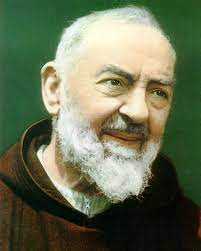
\includegraphics{graphics/Padre_pio.jpeg}

\begin{itemize}
\tightlist
\item
  Save image in reproducible manner
\end{itemize}

\begin{enumerate}
\def\labelenumi{\arabic{enumi}.}
\item
  \begin{itemize}
  \tightlist
  \item
    pdf()
  \item
    code for image
  \item
    dev.off()
  \end{itemize}
\item
\end{enumerate}

\begin{itemize}
\tightlist
\item
  ggsave
\end{itemize}

\hypertarget{table}{%
\subsubsection{Table}\label{table}}

\begin{Shaded}
\begin{Highlighting}[]
\CommentTok{\# kable()}
\FunctionTok{library}\NormalTok{(knitr)}
\FunctionTok{include\_graphics}\NormalTok{(}\StringTok{"graphics/Screen Shot 2022{-}09{-}20 at 11.53.46 PM.png"}\NormalTok{)}
\end{Highlighting}
\end{Shaded}

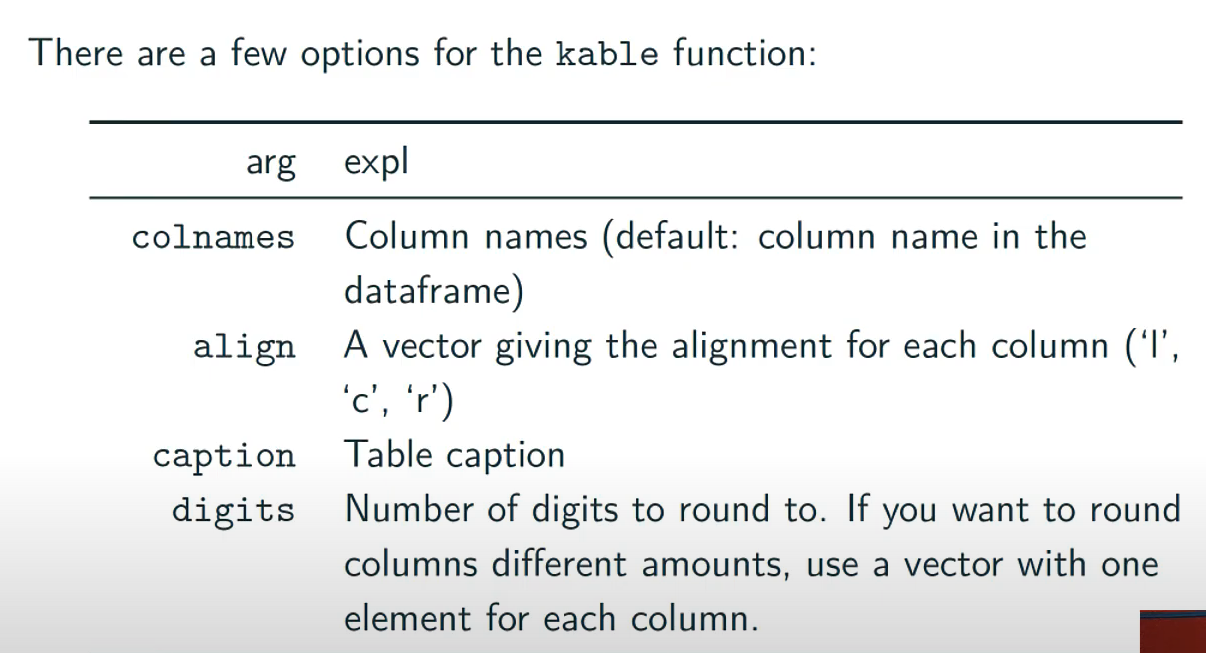
\includegraphics{graphics/Screen Shot 2022-09-20 at 11.53.46 PM.png} \#
R Basics \textbf{na.rm = T} will allow calculations even with NA values.
\textbf{names} (object) \textless- c(``name1'',``name2'') will allow
naming x \textless- c(four=4, five=5, one =1) will name and set in one
step grep(````,a\$?): find'''' within specific row or column which():
returns position subset() or a{[},{]}: returns subset of vector or data
frame paste0(,): paste together two objects

\hypertarget{tidyverse}{%
\section{TidyVerse}\label{tidyverse}}

a \%\textgreater\% \textbf{filter} (all1==``G''): kinda like subset ()
or a{[},{]} \textbf{recode}
(a\(g, `1`='T/T',`2`='A/T',`3`='A/A'): change the way objects are layed out. a %>% **arrange(t)** : like a[order(a
\)t),{]} a \%\textgreater\% \textbf{select}(aff,g): like
a{[},c(``aff'',``all1''){]}

\end{document}
